\documentclass[a4paper,10pt]{article}
\usepackage[a4paper, total={6in, 8in}]{geometry}
\setlength\parindent{0pt}
\usepackage[utf8]{inputenc}
\usepackage{graphicx} 
\usepackage{amsmath}
\usepackage{amsfonts}
\usepackage{amssymb}
\usepackage{listings}
\usepackage{ragged2e}
\usepackage{listings}
\usepackage{color}
\usepackage[table]{xcolor}
\usepackage{soul}
\usepackage[font=small,labelfont=bf]{caption}
\setlength{\parskip}{\baselineskip}%
\setlength{\parindent}{0pt}%

\begin{document}
\begin{titlepage}
	\centering
	
\includegraphics[width=.6\textwidth]{liu-logo.png}\par
	\vfill
	{\scshape\Large TDDD41 Data Mining - Clustering and Association Analysis\par}
	{\huge\bfseries Lab 1 -  Group 4 Report\par}
	\vspace{0.5cm}
    {\large\itshape Lawrence Thanakumar Rajappa (lawra776)\\
     \large\itshape Kyriakos Domanos (kyrdo817)\par}
	\vfill
	{\large \today\par}
\end{titlepage}
\definecolor{dkgreen}{rgb}{0,0.6,0}
\definecolor{gray}{rgb}{0.5,0.5,0.5}
\definecolor{mauve}{rgb}{0.58,0,0.82}

\lstset{frame=tb,
  language=R,
  aboveskip=3mm,
  belowskip=3mm,
  showstringspaces=false,
  columns=flexible,
  basicstyle={\small\ttfamily},
  numbers=none,
  numberstyle=\tiny\color{gray},
  keywordstyle=\color{blue},
  commentstyle=\color{dkgreen},
  stringstyle=\color{mauve},
  breaklines=true,
  breakatwhitespace=true,
  tabsize=3
}
\begin{center}
	\large\textbf{\underline{Clustering}} \par
\end{center}
\textbf{\large\underline{SimpleKmeans}} \par
We have loaded the foods dataset into Weka explorer and found that the dataset contains 27 rows and 6 columns namely;
Name of the foods and corresponding amount of protein, calcium, fat, iron and energy found in the foods. \par
We clustered the data by navigating to \textbf{\textit{Cluster}} tab in the tool. We selected 
\textbf{\textit{SimpleKmeans}} algorithm (with default values i.e. \textbf{number of clusters}:2, \textbf{seed} : 10).
\par
\textbf{1. Choose a set of attributes for clustering and give a motivation. (Hint: always ignore attribute "name". Why does the name attribute need to be ignored?)}\par
We added \textbf{\textit{"Name"}} attribute to the ignore list as it does not provide any value to the analysis and it's just a 
label to the data points. We selected the attributes which are not directly correlated with each other. But choosing
all attributes for the analysis will make our job more complex. First, we chose \textbf{\textit{'protein'}}
and \textbf{\textit{'fat'}} instead of \textbf{\textit{'energy'}} because energy is depending on them. 
Next, we chose \textbf{\textit{'calcium'}}. \par
\textbf{2. Experiment with at least two different numbers of clusters, e.g. 2 and 5, but with the same seed value 10.}\par
We performed clustering with different number of clusters i.e. 2,5,8 but as per theory, with more values of \textbf{'k'}
the k-means algorithm creates non-overlapping subgroups (clusters) where each data point belong to a cluster. We found another significant
information from explorer that as the number of clusters increased \textbf{\textit{'sum of squared errors within cluster'}} decreased.
For example, for \textbf{\textit{k=2}}, the SSE is \textbf{5.069321339929419} and for \textbf{\textit{k=5}}, the
SSE is \textbf{2.750432407251998}. In terms of Machine Learning and Data Analysis, lower value of SSE means the 
analysis or machine learning model is very good and will yield better results. \par
\textbf{3. Then try with a different seed value, i.e. different initial cluster centers. Compare the results with the previous results. Explain what the seed value controls.} \par
We performed clustering with different seed values, but found that if seed value is changed and for higher values of k (k=8), the clusters are unstable.
On the contrary, if k values are less i.e. if k=2 or k=3, the results are almost similar for different seed values.
The seeds are set in weka to initialize the centroids before optimisation starts since k-means doesn't have a global optimum.
Hence, we need to use different seed values and we need to pick the solution based on the lower SSE and also selecting the seed value is arbitrary.
\par
\textbf{4. Do you think the clusters are "good" clusters? (Are all of its members "similar" to each other? Are members from different clusters dissimilar?)} \par
Good clusters depends on what attributes we are selecting. In general, if we have many attributes, it is very hard
to visualize them all at once. Hence visualizing an attribute against itself,we can inspect whether the elements
are falling into the similar clusters. In the below plot, we can see that elements in one cluster are similar to 
one another in terms of calcium and they are dissimilar to other clusters. 
\par
\begin{center}
  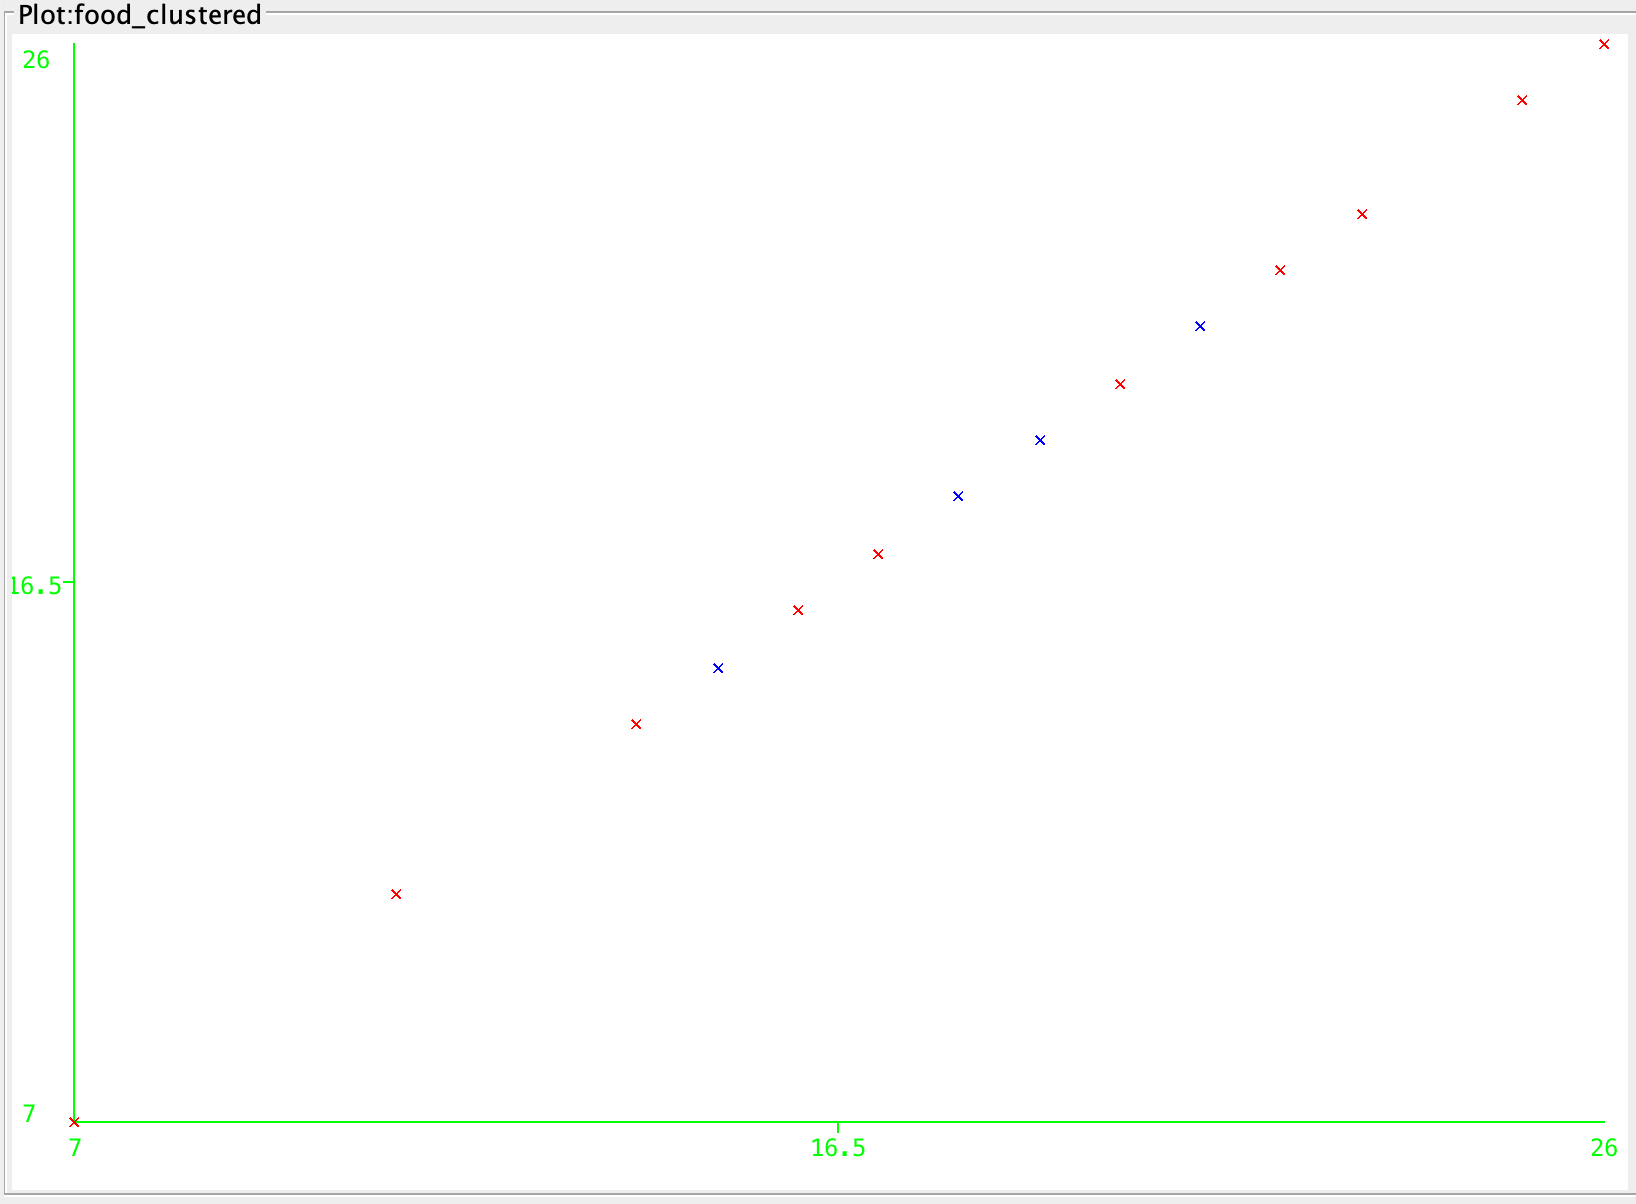
\includegraphics[width=80mm,scale=0.10]{Calcium_Cluster.png}
  \captionof{figure}{The red cluster covers most of the elements when compared with blue cluster, but there tends to be slight overlapping}
\end{center}
\par
\begin{center}
  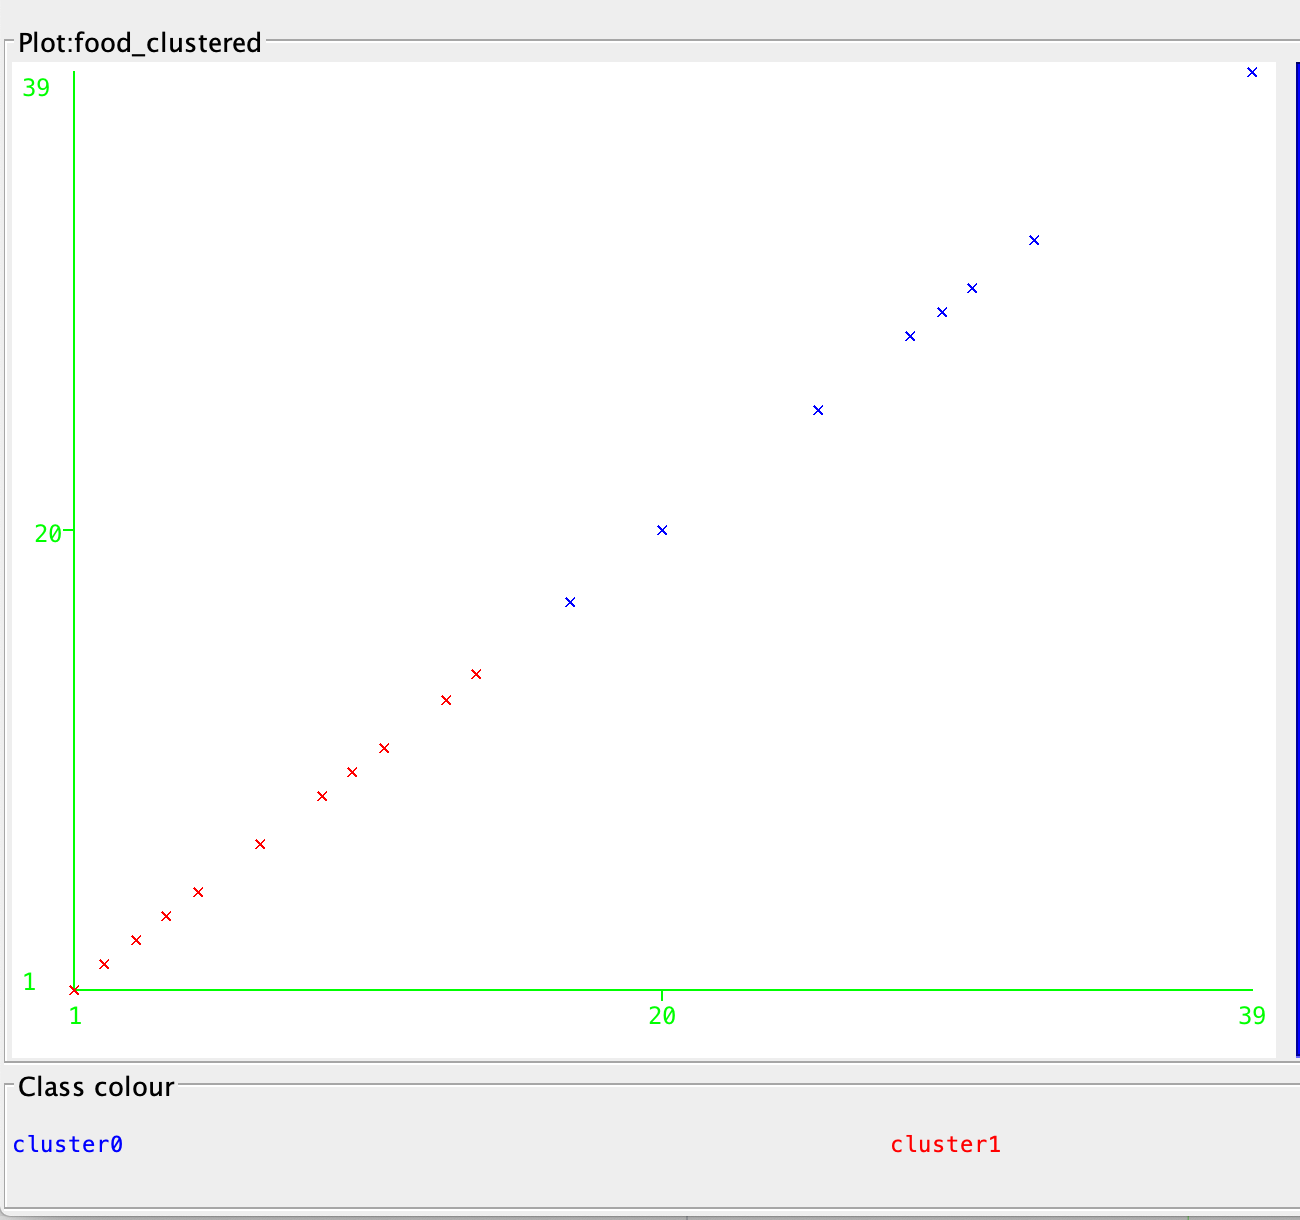
\includegraphics[width=80mm,scale=0.10]{Fat_Cluster.png}
  \captionof{figure}{Blue cluster is having more amount of fat when compared with red cluster. Within-cluster similarity is high}
\end{center}
\par
\begin{center}
  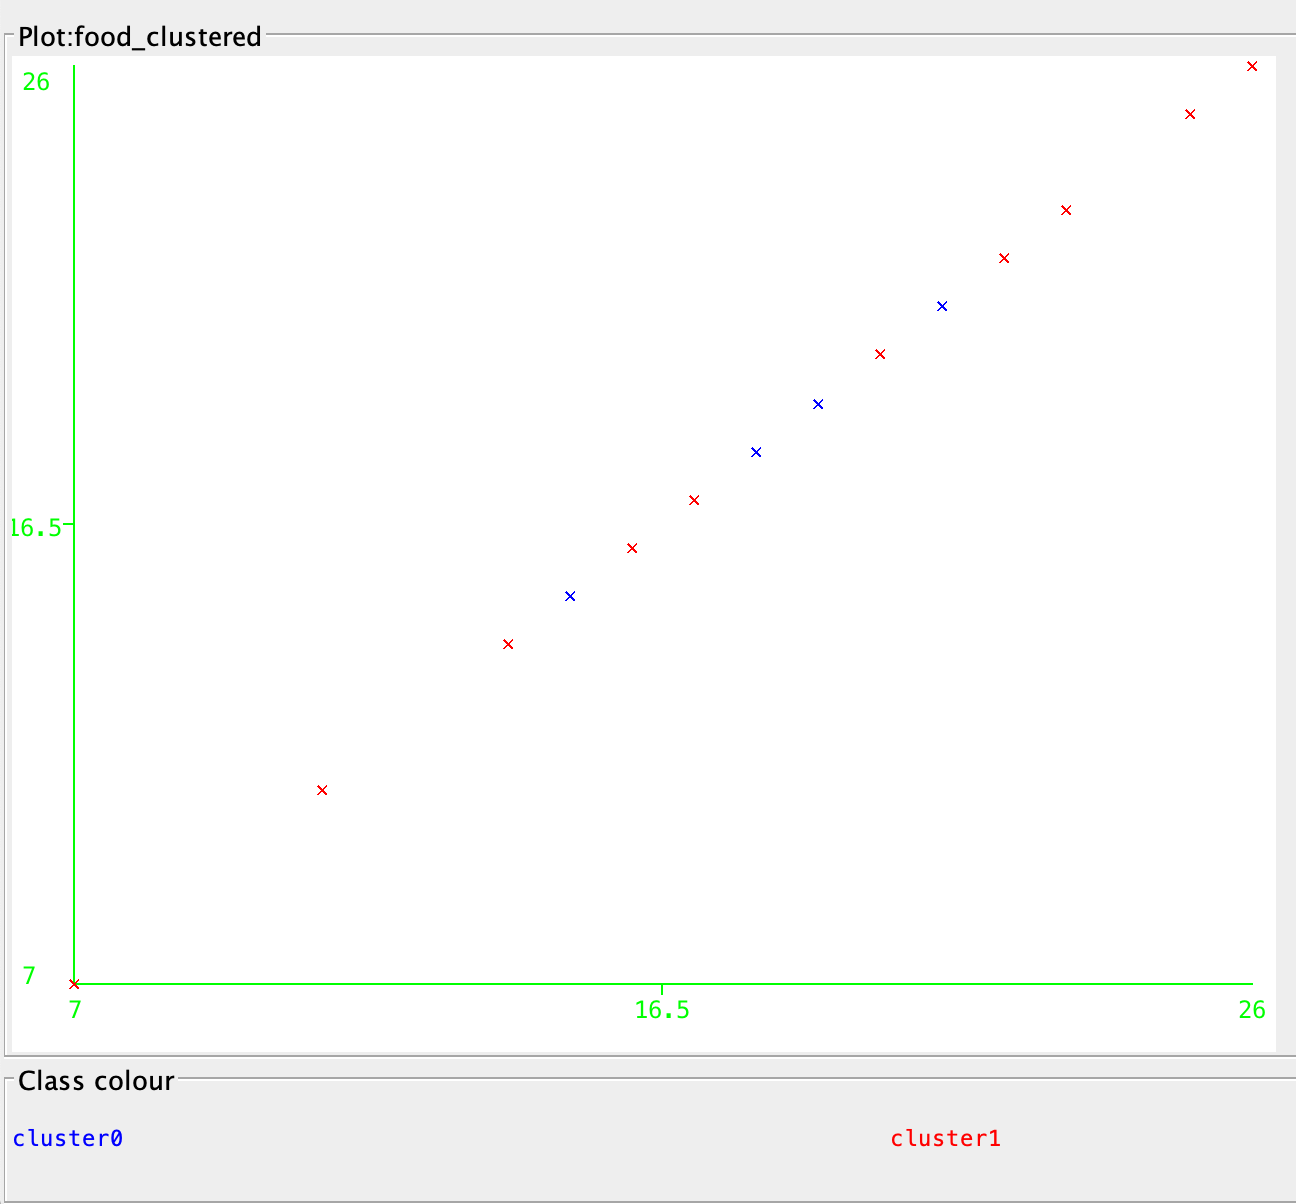
\includegraphics[width=80mm,scale=0.10]{Protein_Cluster.png}
  \captionof{figure}{This clustering is not good because there is more overlapping and hence within-cluster similarity is low}
\end{center}
\par
\textbf{5. What does each cluster represent? Choose one of the results. Make up labels (words or phrases in English) which characterize each cluster.} \par
We have chosen \textbf{\textit{k=2}} with \textbf{\textit{seed=10}}, from the plots above, we can observe that clustering is 
better in terms of \textbf{\textit{'Fat'}}. In particular, we can see that blue cluster meat has higher fat and lower calcium levels while red 
cluster meat has lower fat and higher calcium levels.
\newpage
\textbf{\large\underline{MakeDensityBasedClusters}} \par
\textbf{2. Experiment with at least two different standard deviations. Compare the results.} \par
Standard deviation plays a major role in density based clustering. This method of clustering does not work well if 
there is varying density because the distance threshold $\epsilon$ and minpoints in identifying the neighbourhood points 
will vary as the density varies. This algorithm produces clusters by using k-means and then adjusts the cluster with
small standard deviation. Hence, small standard deviation will provide good number of clusters. But increasing the standard 
deviation results in adding the data points which are dissimilar to the cluster or even there is a possiblity of reducing the 
number of clusters.
We also need to check the inter-cluster distance between a mean of a given attribute and the standard deviation of the 
attribute in order to know the significance in differentiating a cluster. \par
with \textbf{\textit{k=2}}, we used default standard deviation $\sigma=$ 1.0E - 6, we got two clusters and the results were
similar to the results which we obtained in k-means with \textbf{\textit{k=2}}. With $\sigma=$20, when compared with 
$\sigma=$ 1.0E - 6, only one element is shifted in two clusters. with $\sigma=$ 300, all the elements are moved to single 
cluster in order to meet the minimum standard deviation and there are no points outside this cluster.
\end{document}

